% ============================================================
% DIAGRAM: Mixtral Mixture of Experts (2024)
% ============================================================
% Caption: Figure 7.2: Mixtral sparse MoE architecture.
%          (Adapted from Jiang et al., 2024, p. 2)
% ============================================================

\documentclass[tikz,border=10pt]{standalone}
\usepackage{tikz}
\usepackage{amsmath}
\usepackage{amsfonts}

\usetikzlibrary{shapes,arrows,positioning,fit,calc,backgrounds}

\begin{document}

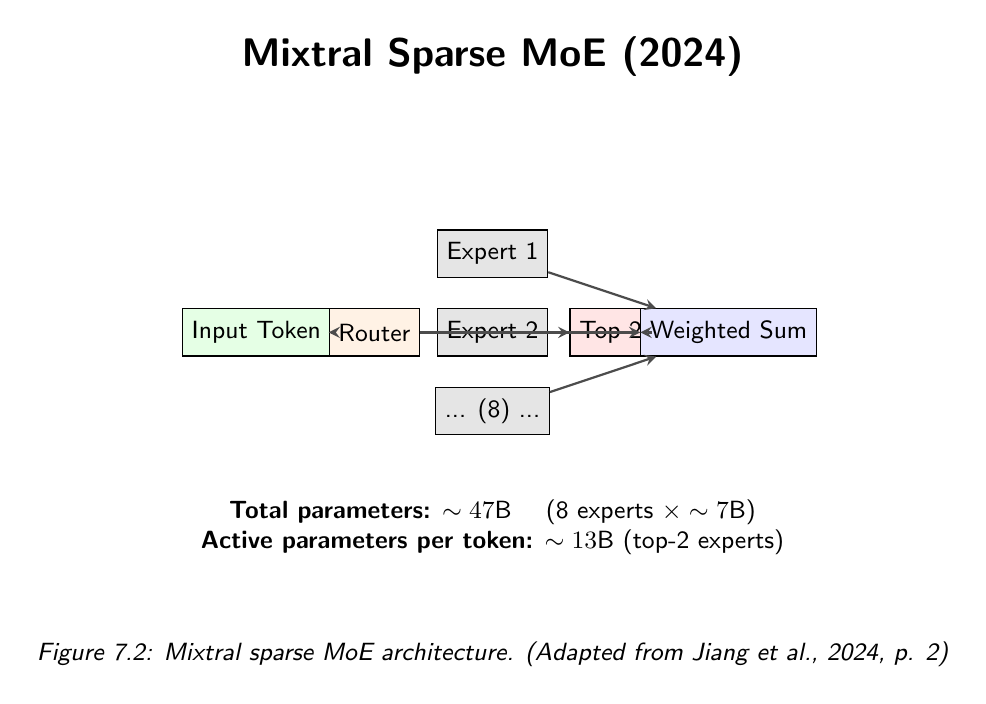
\begin{tikzpicture}[
    block/.style={draw, rectangle, minimum width=0.8cm, minimum height=0.6cm, fill=blue!10, font=\sffamily\small},
    edge/.style={-stealth, thick, draw=black!70},
    label/.style={font=\sffamily\small},
    title/.style={font=\sffamily\Large\bfseries},
    caption/.style={font=\sffamily\small\itshape},
]

\node[title] at (0, 3.5) {Mixtral Sparse MoE (2024)};

% Input token
\node[block, fill=green!10] (input) at (-3, 0) {Input Token};

% Router
\node[block, fill=orange!10] (router) at (-1.5, 0) {Router};

% Experts (8)
\node[block, fill=gray!20] (exp1) at (0, 1) {Expert 1};
\node[block, fill=gray!20] (exp2) at (0, 0) {Expert 2};
\node[block, fill=gray!20] (exp3) at (0, -1) {... (8) ...};

% Top-2 routing
\node[block, fill=red!10] (top2) at (1.5, 0) {Top-2};

% Output
\node[block, fill=blue!10] (out) at (3, 0) {Weighted Sum};

\draw[edge] (input) -- (router);
\draw[edge] (router) -- (top2);
\draw[edge] (top2) -- (out);
\draw[edge] (exp1) -- (out);
\draw[edge] (exp2) -- (out);
\draw[edge] (exp3) -- (out);

% Parameters
\node[align=center, font=\sffamily\small, anchor=north] at (0, -2.0) {
  \textbf{Total parameters:} $\sim 47\text{B}$ \quad (8 experts $\times \sim 7\text{B}$) \\
  \textbf{Active parameters per token:} $\sim 13\text{B}$ (top-2 experts)
};

\node[caption, anchor=north] at (0, -3.8) {
  Figure 7.2: Mixtral sparse MoE architecture. (Adapted from Jiang et al., 2024, p. 2)
};

\end{tikzpicture}
\end{document}
